\chapter{System beskrivelse}
System er beregnet til behandling af patienter med acute ischemic stroke(AIS). Formålet er pre, per og postkonditioning af disse patienter. Systemet skal kunne lave arteriel okklusion i de øverste ydre ekstremiteter. For at sikre tilstrækkelig okklusion, skal det systoliske blodtryk først måles og derefter pumpes manchetten op til plus 25 mmHg over det målte tryk. Som minimum skal der afklemmes med et tryk på 200 mmHg. Okklusionenfasen  bliver holdt konstant i 5 minutter, hvorefter trykket lukkes ud der holdes en \textquotedbl pause\textquotedbl{} på 5 minutter, reperfusionsfasen. Denne proces gentages indtil det antal specificerede cyklusser er kørt. Endvidere kræves det af produktet, at både længden og antallet af okklusionfaser og reperfusionsfaser skal kunne ændres løbende. 
For at sikre at den arterielle afklemning ikke skader patienten, skal produktet kunne indikere om der opnås tilfredsstillende perfusion af det afklemte væv efter okklusionfasen, kaldet \textit{sikkerhedskontrol}. Produktet indbefatter derfor også et pulsoximeter, der efter hver okklusionsfase tjekker kredsløbet. Systemet skal også kunne dokumenterer behandlingsforløbene, og derfor udstyres systemet med ekstern hukommelse, der gør det muligt for bruger at eksportere data og se oversigt over forløbet. 
Som sideløbende krav kan produktet også bruges til okklusionstræning. Her pumpes manchet trykket op til 100 mmHg og det tryk holdes konstant indtil okklusionsættet er færdigt.  

\section{Systemoversigt}
\begin{figure}[H]
	\centering
	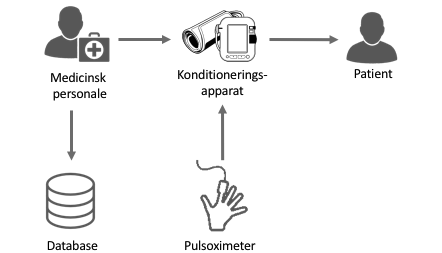
\includegraphics[width=0.8\textwidth]{Kravspecifikation/Illustrationer/saelgertegning.png}
	\caption{Oversigt over systemet, \textit{Konditioneringsapparat}}
\end{figure}
